\documentclass{article}
\usepackage{times}
\usepackage{a4wide}
\usepackage{latexsym}
\usepackage{mathrsfs}
\usepackage{amsmath}
\usepackage{amssymb}
\usepackage{amsthm}
\usepackage{ifthen}
\usepackage{stmaryrd}
\usepackage{algorithm}
%\usepackage{algorithmic}
\usepackage{algpseudocode}
\usepackage{graphics}
\usepackage{epsfig}
\usepackage{graphicx}
\usepackage{subfigure}
% \usepackage[UTF8]{ctex}
%\usepackage{ramacros}
\newtheorem{lemma}{Lemma}[section]

\addtolength{\textwidth}{20mm}
\addtolength{\oddsidemargin}{-10mm}
\addtolength{\textheight}{18mm}
\addtolength{\topmargin}{-9mm}

\newcounter{exercise}
\setcounter{exercise}{0}
\newcommand{\exercise}{
        \addtocounter{exercise}{1}
        \vspace{0.2in}
        \noindent
        {\bf \theexercise .}
        }

\newcommand{\REMARK}[1]{}


\newcommand{\NEWPART}{\vspace{.1in}
              \noindent}

\newcommand{\<}{
    \langle}

\renewcommand{\>}{
    \rangle}

\newcommand{\ceil}[1]{\left\lceil #1 \right\rceil}

\pagestyle{plain} \pagenumbering{arabic}

\title{{\bf Assignment 1} \\ {\large ID: 120037910002 } {\large Name: Xingguo Jia } {\large Email: jiaxg1998@sjtu.edu.cn}}

\author{}
\date{}

\begin{document}
\maketitle

%{\large \noindent
%\begin{tabular}{lcl}
%{Jan 17 2007}.
%\end{tabular}
%}

{\large





\begin{exercise}
Prove the K\"onig theorem: Let $G$ be bipartite, then cardinality of maximum matching = cardinality of minimum vertex cover.

\end{exercise}
\begin{proof} 
    \leavevmode\newline
\begin{itemize}

\item We define $L$ to be the left part of $G=(V,E)$ and $R$ to be the right part, and suppose we have $M$ to be the maximum matching. Start from a vertex in $R$ that is not a vertex of any edge in $M$, we go through a path (not in $M$) $\rightarrow$ (in $M$) $\rightarrow$  (not in $M$) $\rightarrow$ (in $M$) $\ldots$ until the path cannot continue(alternating path). 

\item \textbf{All vertices in this path } form a vertex set $U$. \textbf{All edges in this path} form a edge set $P$. This path starts at a vertex in $R$ and ends at a vertex in $R$. Firstly we prove that $m=(L \cap U) \cup (R \setminus U)$ is a \textbf{vertex cover}.

\item We prove by contradiction. Suppose $e \in E$'s right vertex $r$ is in $R\cap U$ and left vertex $l$ is in $L\setminus U$. $e\notin M$ because it shares a vertex $r\in R\cap U$ with an edge $f\in M \cap P$. Then, since $e \notin M$, we have a path from $f$ to $e$ that becomes a part of an alternating path, which is a contradiction.

\item Next we prove that $|m| = |M|$. For each $k \in M \cap P$, it has a vertex in $L\cap U$ corresponding to it. For each $k \in M \setminus P$, its right vertex must $\in R \setminus U$, or it would become part of the path.

\item Finally, $m$ must be the minimum cover. If we remove a vertex $v$ from $m$, then $e \in M$ corresponding to $v$ cannot be covered. 
\end{itemize}
\end{proof}


\begin{exercise}
Consider the algorithm \textbf{Negative-Dijkstra} for computing shortest paths through graphs with negative edge weights (but without negative cycles)
\begin{algorithm}[htb]
\caption{Algorithm 1: Negative-Dijkstra(G,s)}
\begin{algorithmic}[1]
\State $w^*\leftarrow$ minimum edge weight in $G$;
\For{$e\in E(G)$}
\State $w'(e)\leftarrow w(e)-w^*$
\EndFor
\State $T\leftarrow$\textbf{Dijkstra}$(G',s)$; \\
\Return weights of $T$ in the original $G$;
\end{algorithmic}
\end{algorithm}
Note that \textbf{Negative-Dijkstra} shifts all edge weights to be non-negative(by shifting all edge weights by the smallest original value) and runs in $O(m+\log n)$ time.\\
Prove or Disprove: \textbf{Negative-Dijkstra} computes single-source shortest paths correctly in graphs with negative edge weights. To prove the algorithm correct, show that for all $u\in V$ the shortest $s-u$ path in the original graph is in $T$. To disprove, exhibit a graph with negative edges, with no negative cycles where \textbf{Negative-Dijkstra} outputs the wrong "shortest" paths, and explain why the algorithm fails.
\end{exercise}

\textbf{Disprove:}

\begin{figure}[!htp]
    \centering
    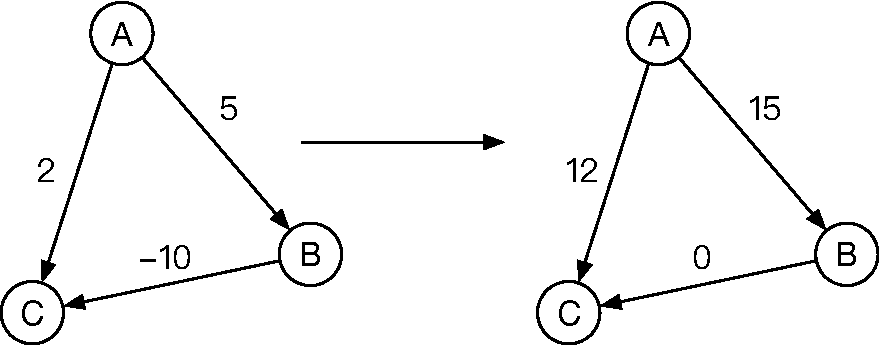
\includegraphics[width=0.5\textwidth]{img/2.pdf}
    \caption{Negative to Non-negative Edges}
    \label{fig:2}
  \end{figure}
See Figure \ref{fig:2}, we shift the graph $G=$ \{$w_{AB}=5,w_{BC}=-10,w_{AC}=2$ \} to $G'=$\{$w_{AB}=15,w_{BC}=0,w_{AC}=12$ \}.
    \begin{itemize}
        \item Use Dijkstra's Algorithm on $G'$, $A$ is the source vertex. Then the shortest path from $A$ to $C$ is 12, after shifting back, it is -2 ($A\rightarrow C$).
        \item Use Dijkstra's Algorithm on $G$, then the shortest path from $A$ to $C$ is -5 ($A\rightarrow B \rightarrow C$), not -2.
        \item Negative-Dijkstra fails because the \textbf{shifting} operation can shift different \textbf{weight} even for the two paths with the same length. The \textbf{more edges} a path has, the more \textit{shift} it gets. It is unfair.
    \end{itemize}


\begin{exercise}
Consider a weighted, directed graph $G$ with $n$ vertices and $m$ edges that have integer weights. A graph walk is a sequence of
not-necessarily-distinct vertices $v_1,v_2,\ldots,v_k$ such that each pair of consecutive vertices $v_i,v_{i+1}$ are connected by an edge. This is similar to a path, except a walk can have repeated vertices and edges. The length of a walk in a weighted graph is the sum of the weights of the edges in the walk. Let $s,t$ be given vertices in the graph, and $L$ be a positive integer. We are interested counting the number of walks from $s$ to $t$ of length exactly $L$.
\begin{itemize}
\item Assume all the edge weights are positive. Describe an algorithm that computes the number of graph walks from $s$ to $t$ of length exactly $L$ in $O((n+m)L)$ time. Prove the correctness and analyze the running time
\item Now assume all the edge weights are non-negative(but they can be 0), but there are no cycles consisting entirely of zero-weight edges. That is, for any cycle in the graph, at least one edge has a positive weight.\\
Describe an algorithm that computes the number of graph walks from $s$ to $t$ of length exactly $L$ in $O((n+m)L)$ time. Prove correctness and analyze running time.
\end{itemize}
\end{exercise}

\textbf{Solution:} We use Dynamic Programming to calculate the number of walks of length exactly $L$. 
    \begin{itemize}
        \item Define $nw(v,l)$ to be the number of walks from vertex $s$ to $v$ of length exactly $l$ ($nw$ stands for \textbf{N}umber of \textbf{W}alks). We need to calculate $nw(t,L)$, where
        \item $nw(v,l)=\sum\limits_{\{u\mid (u,v)\in E,w(u,v)\leq l\}}nw(u,l-w(u,v))$
    \end{itemize}

\begin{algorithm}[htb]
    \label{algo:sss}
    \caption{Number of walks from $s$ to $t$ of length exactly $L$}
    \begin{algorithmic}[1]
        \label{algo:1}
        \For{$v\in V$}
            \For{$l$ from 0 $\rightarrow$ $L$}
                \State $nw(v,l)\leftarrow 0$
            \EndFor
        \EndFor
        
        \State
        \State $nw(s,0)\leftarrow 1$
        
        \label{algo:3}

        \For{$l$ from 0 $\rightarrow$ $L$}
        \label{algo:2}
            \For{$v\in V$}
                \For{$u\in \{u\mid (u,v)\in E,w(u,v)\leq l\}$}
                    \State $nw(v,l)\leftarrow nw(v,l)+nw(u,l-w(u,v))$ 
                \EndFor
            \EndFor
        \EndFor
    \end{algorithmic}
\end{algorithm}

\begin{itemize}
    \item For $G$ with \textbf{zero weight} edges, we remove all edges in $E$ that has positive weight and get $G'$. On line \ref{algo:1}, when setting the initial value of matrix $w(v,l)$, instead of setting them all to $0$, we first run the algorithm on $G'$ to initialize the matrix $w(v,l)$.
    \item On line \ref{algo:2}, it traverses \textbf{no more than} all vertices and edges, which needs $O(n+m)$ time. On line \ref{algo:3}, it runs line \ref{algo:2} for $L$ times. Finally, algorithm \ref{algo:sss} runs in $O((n+m)L)$ time.
\end{itemize}



\begin{exercise}
The diameter of a connected, undirected graph $G=(V,E)$ is the length (in number of edges) of the longest shortest path between two nodes. Show that is the diameter of a graph is $d$ then there is some set $S\subseteq V$ with $|S|\leq n/(d-1)$ such that removing the vertices in $S$ from the graph would break it into several disconnected pieces.

\end{exercise}
\begin{proof} 
    \leavevmode\newline

We use \textbf{Menger's theorem:} Let $G$ be a finite undirected graph and $x$ and $y$ two distinct vertices. Then the size of the minimum edge cut for $x$ and $y$ is equal to the maximum number of pairwise edge-independent paths from $x$ to $y$.
\begin{itemize}
    \item Suppose $x,y\in G$ is the two ends of the diameter of $G$. According to \textbf{Menger's theorem}, the size of the minimum edge cut $S$ for $x$ and $y$ is equal to the maximum number of pairwise edge-independent paths from $x$ to $y$.
    \item The maximum number of pairwise edge-independent paths from $x$ to $y$ is $m$, then $m=|S|$, and $m*(d-1)+2\leq n\implies |S|\leq (n-2)/(d-1) \implies |S| < n/(d-1)$, where removing the vertices in $S\subseteq V$ from the graph would break it into \textbf{two} disconnected pieces.
\end{itemize}

\end{proof}




\begin{exercise}
Let $G$ be a $n$ vertices graph. Show that if every vertex in $G$ has degree at least $n/2$, then $G$ contains a Hamiltonian path.
\end{exercise}
\begin{proof} This is \textbf{Dirac's theorem}, which is weaker than Ore's theorem. Now we just need to prove \textbf{Ore's theorem}: Let $G$ be a (finite and simple) graph with $n \geq 3$ vertices. If $deg(u)+deg(v) \geq n$ for every pair of distinct non-adjacent vertices $u$ and $v$ of $G$, then $G$ is Hamiltonian.
    
    \begin{figure}[!htp]
        \centering
        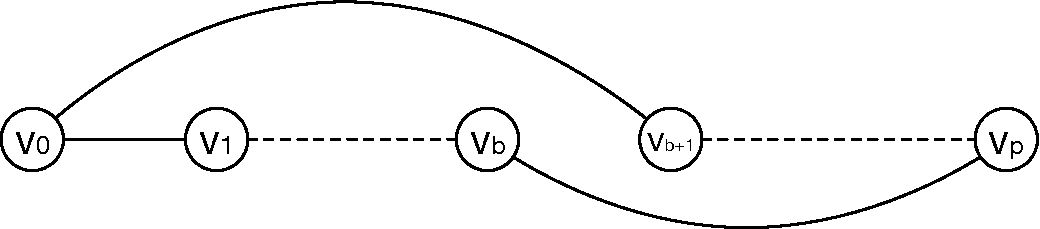
\includegraphics[width=0.6\textwidth]{img/3.pdf}
        \caption{Ore's theorem}
        \label{fig:3}
      \end{figure}
    \begin{itemize}
        \item Firstly, we prove that $G=(V,E)$ must be \textbf{connected} by contradiction. Suppose $V_1$ and $V_2$ are the two sets of disconnected vertices in $V$ and $|V_1|+|V_2|=|V|=n$. WLOG, $|V_1| \leq n/2 \leq |V_2|$. Then, for two vertices $v_1,v_2 \in V_1$, we have $deg(v_1)+deg(v_2) \leq (n/2-1)*2 < n$, which is a contradiction.
        
        \item Suppose path $P=v_0 v_1 \ldots v_p(p\leq n-1)$ is the \textbf{longest} path that does not go through a same vertex more than once. Suppose $v_{i_0},v_{i_1},\ldots,v_{i_k}$ are all vertices adjacent to $v_0$, then they are all on path $P$ and $k\leq p$, \textbf{or} path $v_{i_x}v_0v_1\ldots v_p(0\leq x\leq k)$ is longer than $P$, which is a contradiction. Thus, $deg(v_0)=k+1$.
        
        \item Also, at least one of $v_{i_0},v_{i_1},\ldots,v_{i_k} (k\leq p)$ is adjacent to $v_p$. \textbf{Or}, $deg(v_p)\leq p-(k+1)\implies deg(v_0)+deg(v_p)\leq k+1+(p-(k+1))=p\leq n-1$, which contradicts with $deg(u)+deg(v) \geq n$. Thus, $\exists v_b$ on path $P$ that is both adjacent to $v_0$ and $v_p$. Since $v_b$ and $v_{b+1}$ are adjacent, so we have a Hamiltonian cycle $v_0 \ldots v_b v_p \ldots  v_{b+1} v_0$ in Figure \ref{fig:3}, which has a length of $p+1$.
        
        \item Suppose $p+1 < n$, then $\exists v_m \in G$ is not in path $P$. Since $G$ is \textbf{connected}, $v_m$ can go to a vertex $v_n\in P$ through some path. If $0\leq n\leq b$, then path
        \item $v_m \ldots  v_n v_{n-1} \ldots  v_0 v_{b+1} \ldots  v_{p} v_{p-1} \ldots  v_{b} v_{b-1} \ldots  v_{n+1}$ 
        \item becomes a at least $(p+1)$-long path, which contradicts with the longest path $P$. For $b+1\leq n\leq p$ we have similar contradiction. 
        \item Thus, we have $p+1 \geq n\implies p\geq n-1$, and $p \leq n-1$ since $P \subseteq V$, finally $p=n-1$, which means path $P$ is a Hamiltonian path.
    \end{itemize}
    
\end{proof}




\begin{exercise}
Show how to find a minimal cut of a graph (not only the cost of minimum cut, but also the set of edges in the cut).
\end{exercise}

\textbf{Solution1:}

    \begin{itemize}
        \item Let $G=(V,E)$ be a weighted undirected graph. For two vertices $s,t\in V$, there are two possible situations: global minimum cut of $G$ is also $s-t$ min-cut, or $s$ and $t$ belong to the same side of the global min-cut.
        \item In the latter situation, the global min-cut can be found by merging $s$ and $t$. $G$ becomes $G'=G\setminus \{s,t\}\cup \{st\}$, where $st$ is a vertex representing merged $s$ and $t$. If edge $s-t\in E$, then it disappears. For a vertex $v\in V$ that have an edge to both $s$ and $t$, then $w(v,st)=w(v,s)+w(v,t)$. Return the cut-set of the final state. Run the algorithm recursively on $G'$, and the min-cut of $G'$ is equal to that of $G$.
        
    \end{itemize}
\begin{algorithm}[htb]
    \caption{Stoer-Wagner Algorithm}
    \begin{algorithmic}[1]
        \Procedure{MinCutPhase}{$G=(V,E),a$}
            \State $S \leftarrow \{a\}$
            \While{$|S| < |V|$}
                \State  $w(A,z)=\max\{w(A,y)\mid y\notin A\}$
                \State where $w(A,y)$ is the sum of the weights of all the edges between A and y.
                \State $S\leftarrow S\cup \{z\}$
                \State shrink $G$ by merging the two vertices $(s, t)$ added last.
                \State
                \Return \{cut-of-phase, cut-set\}=$w(A, last-two-vertices)$, cut-set
            \EndWhile      
        \EndProcedure
        \State
        \Procedure{MinCut}{$G=(V,E),a$}
            \While{$|V| > 1$}
                \State \{cut-of-phase,\ cut-set\}$\leftarrow MinCutPhase(G=(V,E),a)$
                \State
                \If{$mincut > $cut-of-phase}
                    \State $mincut \leftarrow\ $cut-of-phase
                    \State $mincutset \leftarrow\ $cut-set
                \EndIf
            \EndWhile
        \EndProcedure
    \end{algorithmic}
\end{algorithm}

\textbf{Solution2:}
\begin{itemize}
    \item Let vertex $s$ to be the source, we run Ford-Fulkerson Algorithm on $G$, and remove all edges that has the max flow to get $G'$.
    \item Run DFS to traverse $G'$, mark all visited vertex to be in $V' \subseteq V$. Then all edges between vertex sets $V'$ and $V\setminus V'$ form the minimum cut.
\end{itemize}


\begin{exercise}
Let $G(V,E)$ be a connected undirected graph with a weight $w(e)>0$ for each edge $e\in E$. For any path $P_{u,v}=<u,v_1,v_2,\ldots,v_r,v>$ between two vertices $u$ and $v$ in $G$,let $\beta(P_{u,v})$ denote the maximum weight of an edge in $P_{u,v}$. We refer to $\beta(P_{u,v})$ as the \textbf{bottleneck weight} of $P_{u,v}$. Define
\begin{displaymath}
\beta^*(u,v)=\min\{\beta(P_{u,v}):P_{u,v}\text{ is a path between $u$ and $v$}\}.
\end{displaymath}
Give a polynomial algorithm to find $\beta^*(u,v)$ for each pair of vertices $u$ and $v$ in $V$ and a proof of the correctness of the algorithm.
\end{exercise}

\textbf{Solution:}
    \begin{itemize}
        \item We say a \textbf{minimum bottleneck spanning tree (MBST)} is a spanning tree that minimizes the most expensive edge. First we prove that \textbf{MST} must be a MBST. If not, consider the most expensive edge $e_1$ of MST and most expensive edge $e_2$ of MBST, we have $w(e_1)>w(e_2)$. Then, we replace $e_1$ from MST with $e_2$, then we have a spanning tree that has smaller weight than MST, which is a contradiction.
        \item Similarly, we can prove by contradiction that a minimum bottleneck path must be on \textbf{MST}. So, we first get MST by running \textbf{Prim Algorithm}. Then, for each pair of vertices $u$ and $v$, we do a DFS from $u$ to $v$ to find the minimum bottleneck path, then we get $\beta^*(u,v)$.
    \end{itemize}



\begin{exercise}
Let $G=(V,E)$ be a directed graph. Give a linear-time algorithm that given $G$, a node $s\in V$ and an integer $k$ decides whether there is a walk in $G$ starting at $s$ that visits at least $k$ distinct nodes.
\end{exercise}
\textbf{Solution:} 
    \begin{itemize}
        \item Use Tarjan Algorithm to get all \textbf{Strongly Connected Components (SCC)} of $G$. In A \textbf{SCC} there is a path that goes through each vertex in SCC for at least once.
        \item Define $G'=(V', E')$ where each $v\in V'$ corresponds to an SCC of $G$, and for each edge $(u\rightarrow v) \in E'$, $w(u\rightarrow v)=|GCC(v)|$, where \textbf{GCC(v)} is the GCC in $G$ corresponding to $v$.
        \item Suppose $s$ is in $GCC(s')$. We do a DFS starting at $s'$ in $G'$. We set $w\leftarrow 0$. When getting to a vertex $t'$, $w\leftarrow w+w(t')$. If $w>=k$, return $true$. If DFS is done, return $false$.
        \item Time complexity is $O(|V|+|E|)$, which is linear to $V$ and $E$.
    \end{itemize}




\begin{exercise}
\textbf{Minimum Bottleneck Spanning Tree}: Given a connected graph $ G $ with positive edge costs, find a
spanning tree that {minimizes the most expensive edge}.
\end{exercise}

\textbf{Solution:}
\begin{algorithm}[htb]
    \caption{Camerini's Algorithm}
    \begin{algorithmic}[1]
        \Procedure{MBST}{$G=(V,E)$}
        \If{$|E|=1$}
        \State
        \Return $E$
        \EndIf
        \State
        \State $E_1=\{e\in E \mid w(e) > w_m\}$, $E_2=\{e\in E \mid w(e) \leq w_m\}$, $A=(E_1, V_1)$, $B=(E_2, V_2)$
        \State $|F| \leftarrow$ spanning tree (forest) of B
        \State
        \If $|F| = 1$
            \State return MBST$(B)$
        \Else
            \State $V'\leftarrow$ contract each connected component in B into a single vertex
            \State $E'\leftarrow$ edges in A that connect the connected components in B
            \State
            \Return $F \cup (V', E')$ 
        \EndIf
        \EndProcedure
    \end{algorithmic}
\end{algorithm}
    \begin{itemize}
        \item Suppose we need to find an \textbf{MBST} (Minimum Bottleneck Spanning Tree) in a undirected, connected, positive edge-weighted graph $G=(V,E)$. We have Camerini's Algorithm to find such a MBST in $O(n)$ time, which works as follows.
        \item Find the \textbf{median} edge weight $w_m$ in $E$, then partition $E$ into $E_1=\{e\in E \mid w(e) > w_m\}$ and $E_2=\{e\in E \mid w(e) \leq w_m\}$.
        \item Define $F$ to be the spanning tree forest of $E_2$. If $|F|=1$ then run the former step on $B$. 
        \item Else, contract each connected component in $B$ to a single vertex. Create a new graph by using all vertices from the contraction ($V'$), and all edges in $A$ that connects the connected components in $B$ ($E'$). We have $|V'|=|F|$, $G'=(V',E')$, MBST is $F \cup MBST(G')$.
        \item This algorithm works in $O(E/2)+O(E/4)+O(E/8)+\ldots =O(E)$ time.
    \end{itemize}


\end{document}
